% !TEX program = xelatex

\documentclass[no-math,twoside]{exam}  %不含答案
\newcommand{\new}{}
\usepackage{xeCJK}%使用xeCJK中文处理宏包
\usepackage{CJKfntef}
\usepackage{CJKnumb}%中文小写数字
\usepackage{amsmath,amssymb}%ams数学符号
\usepackage{calc}%使用四则运算宏包
\usepackage{intcalc}%使用mod,感谢qingkuan大神指导
\usepackage{ifthen}%使用条件判断宏包
\usepackage{zref-user}
\usepackage{zref-lastpage}%使用zref宏包,引用数字标签值和LastPage标签,感谢qingkuan大神指导
%\usepackage{refcount}%使用refcount宏包,引用数字标签值,已改用zref宏包实现,感谢qingkuan大神指导
\usepackage{makecell}
\usepackage{interfaces-makecell}%使用interfaces-makecell宏包,制作列数可变表格,感谢qingkuan大神指导
\usepackage{dashrule}%使用虚线宏包
\usepackage{parskip}%段落无缩进宏包
\usepackage{graphicx}%使用图形包
%\usepackage{color}%使字体颜色
\usepackage{esvect}%与教材向量符号相同
\usepackage{cases}%方程组
\usepackage{CJKfntef}%着重号
\usepackage{yhmath} %弧
\usepackage{mathptmx}
\usepackage{anysize}
\usepackage{enumitem}
\usepackage{tikz}
\usepackage[Symbol]{upgreek}
\usepackage{bm}
%====================================================================================================%
%
%
%====================================================================================================%
\setmainfont{Times New Roman}
\setmonofont{FZSSJW--GB1-0}
\newcommand{\heiti}{\CJKfontspec{STHeitiSC-Light}}%adobe 黑体
\newcommand{\fs}{\CJKfontspec{FangSong}}%adobe 仿宋
\newcommand{\kai}{\CJKfontspec{Kai}}%adobe 楷体

\usepackage[left=18mm,right=18mm,top=18mm,bottom=18mm,includefoot]{geometry}


%\setmainfont{Minion Pro}
%\setmathfont{Asana Math}




%\usepackage{tabularx}
\usepackage{tabu}
\usepackage{graphicx}
%\usepackage{picins}
\usepackage{siunitx}
\renewcommand{\baselinestretch}{1.3} %必要可调整行距

%\usepackage[paperheight=297 true mm,paperwidth=210 true mm, top=15 truemm,bottom=25 true mm,left=24 true mm,right=24 true mm, headsep=-20pt]{geometry}

%\usepackage
%[paperheight=132 true mm,paperwidth=176 true mm, top=5 true
%mm,bottom=15 true mm,left=5 true mm,right=10 true mm, headsep=-20pt]
%{geometry}
%\usepackage{hyperref}
%\hypersetup{pdfpagemode={FullScreen},pdfencoding=unicode}



%\usepackage{fancyhdr}%使用页眉页脚宏包
%\pagestyle{fancy}
%
%用到的长度变量
%\newlength{\wot}%所有表格每列宽度
%\newlength{\wol}%所有横线的宽度
%\newlength{\gmw}%gutter margin width 装订线页眉外侧超宽位置
%\newlength{\dl}%dash length横线长
%

%页眉设置开始
%\pagestyle{fancy}                    % 设置页眉
%\lhead{\logo{\includegraphics[height=8.5 mm]{logo1.png}}}
%\lhead{\logo{\includegraphics[height=8.5 mm]{logo2.png}}}
%\lhead{\bfseries \heiti 高考数学重点知识扫描}}
%\rhead
%{{  {\heiti 高一教学资料}}}


%===============
%双线页眉的设置
%\makeatletter %双线页眉
%\def\headrule{{\if@fancyplain\let\headrulewidth\plainheadrulewidth\fi%
%\hrule\@height 1.0pt \@width\headwidth\vskip1pt%上面线为1pt粗
%\hrule\@height 0.5pt\@width\headwidth  %下面0.5pt粗
%\vskip-2\headrulewidth\vskip-1pt}      %两条线的距离1pt
  %\vspace{6mm}}     %双线与下面正文之间的垂直间距
%\makeatother
%===============%页眉设置结束     
\newlength{\lab}
\newlength{\lb}
\newlength{\lc}
\newlength{\ld}
\newlength{\lhalf}
\newlength{\lquarter}
\newlength{\lmax}
\newcommand{\xx}[4]{\\[.5pt]%
  \settowidth{\lab}{A.~#1~~~}
  \settowidth{\lb}{B.~#2~~~}
  \settowidth{\lc}{C.~#3~~~}
  \settowidth{\ld}{D.~#4~~~}
  \ifthenelse{\lengthtest{\lab > \lb}}  {\setlength{\lmax}{\lab}}  {\setlength{\lmax}{\lb}}
  \ifthenelse{\lengthtest{\lmax < \lc}}  {\setlength{\lmax}{\lc}}  {}
  \ifthenelse{\lengthtest{\lmax < \ld}}  {\setlength{\lmax}{\ld}}  {}
  \setlength{\lhalf}{0.5\linewidth}
  \setlength{\lquarter}{0.25\linewidth}
  \ifthenelse{\lengthtest{\lmax > \lhalf}}  {\noindent{}A.~#1 \\ B.~#2 \\ C.~#3 \\ D.~#4 }  {
  \ifthenelse{\lengthtest{\lmax > \lquarter}}  {\noindent\makebox[\lhalf][l]{A.~#1~~~}%
    \makebox[\lhalf][l]{B.~#2~~~}\\%
    \makebox[\lhalf][l]{C.~#3~~~}%
    \makebox[\lhalf][l]{D.~#4~~~}}%
    {\noindent\makebox[\lquarter][l]{A.~#1~~~}%
      \makebox[\lquarter][l]{B.~#2~~~}%
      \makebox[\lquarter][l]{C.~#3~~~}%
      \makebox[\lquarter][l]{D.~#4~~~}}}}

\newcommand{\kh}[1][0.7]{\nolinebreak\hfill%\dotfill
\mbox{%\raisebox{-1.8pt}
  % {$\cdots$}
   (\hspace{#1 cm})}%\\
   }
%****************圆弧  $\overparen{ABCDE}$****************
%定义圆弧  %$\wideparen{ABCDE}$
\DeclareSymbolFont{ugmL}{OMX}{mdugm}{m}{n}
\SetSymbolFont{ugmL}{bold}{OMX}{mdugm}{b}{n}
\DeclareMathAccent{\wideparen}{\mathord}{ugmL}{"F3}


%****************平行****************
\renewcommand\parallel{%               %平行
	\mathrel{\text{\tikz[baseline]
			\draw (0em,-0.3ex) -- (.4em,1.7ex)
			(.2em,-0.3ex) -- (.6em,1.7ex);%
}}}
%带圈数字
\newcommand{\dqsz}[1]
{\unitlength=1mm\begin{picture}(4.8,3.4)(-2.4,-1.4)
	\put(0,0){\makebox(0,0){\scalebox{0.9}{#1}}}
	\put(0,0){\circle{3.4}}
	\end{picture}}

            
%%%%%%%%%%%%%%%%%%%%%%%%%%%%%%%%%%%%%%%%%%%%%%%%%%
%****************圆弧  $\overparen{ABCDE}$****************
%定义圆弧  %$\wideparen{ABCDE}$
\DeclareSymbolFont{ugmL}{OMX}{mdugm}{m}{n}
\SetSymbolFont{ugmL}{bold}{OMX}{mdugm}{b}{n}
\DeclareMathAccent{\wideparen}{\mathord}{ugmL}{"F3}

\newcommand*\congruent{%                                       %全等
    \mathrel{\text{%
    \tikz \draw[baseline] (-.22em,-.4ex) arc (-90:-285:0.4ex) (-.22em,-.4ex) .. controls (0,-.4ex) and (0,.4ex) .. (.22em,.4ex) arc (90:-105:0.4ex) (-.4em,-.75ex) -- (.4em,-.75ex) (-.4em,-1.1ex) -- (.4em,-1.1ex);%
}}}

%%%%%%%%%%%%%%%%%%%%%%%%%%%%%%%%%%%%%%%%%%%%%%%%%%
\renewcommand{\solutiontitle}{{\bfseries 答案:}}

\renewcommand\thepartno{\arabic{partno}}
\renewcommand\thesubpart{\roman{subpart}}
\renewcommand\subpartlabel{(\thesubpart)}
%\renewcommand\thepartno{\Roman{partno}}
%\renewcommand\thepartno{\Alph{partno}}
%\renewcommand\thepartno{\Greeknum{partno}}

\newcommand{\envert}[1]{\left\lvert#1\right\rvert}
\let\abs=\envert
%以上定义绝对值, 用法: \abs{ }
\newcommand\set[1]{\left\{\rule{0cm}{1.7ex} {#1} \right\}}
%定义列举法集合表示
\newcommand\Set[2]{\left\{\rule{0cm}{1.7ex}\, {#1} \, \middle\vert \, {#2} \,\right\}}
%定义描述法集合表示
\newcommand{\dt}{\,\symup{d} t}
\newcommand{\dx}{\,\symup{d} x}
\newcommand{\dy}{\,\symup{d} y}
\newcommand{\dint}{\displaystyle\int}

\usepackage{esvect}
\renewcommand{\vec}{\vv}

%定义平行且相等
\usepackage{pict2e}
\newcommand\paralleleq{%
  \begingroup
  \setlength\unitlength{0.1em}%
  \linethickness{0.5\unitlength}%
  \roundcap
  \mathrel{\begin{picture}(6,7)
    \Line(0,-1)(6,-1)
    \Line(0,0.5)(6,0.5)
    \Line(1.5,1.5)(3.5,7)
    \Line(3.5,1.5)(5.5,7)
  \end{picture}}
  \endgroup}


%圆弧  
%$\overparen{ABCDE}$
%****************定义平行四边形\parallelogram  ****************
\newcommand*\paralogram{%            %平行四边形parallelogram  
  \mathord{\text{%
    \tikz[baseline]
      \draw (0,.1ex) -- (.8em,.1ex) -- (1em,1.4ex) -- (.2em,1.4ex) -- cycle;}}}

%解决 \underbrace 和 \overbrace 的问题
%用法: $\underset{\text{共$n$个}}{ \underbrace {333\cdots333}}$

\XeTeXcharclass `①=1
\XeTeXcharclass `②=1
\XeTeXcharclass `③=1
\XeTeXcharclass `④=1
\XeTeXcharclass `⑤=1
\XeTeXcharclass `∥=1
\XeTeXcharclass `▲=1

%\renewcommand{\figurename}{图}

%\newcommand\df[1]{\quad\dotfill~#1~分}
%\newcommand\df[1]{\hbox{}\nobreak\dotfill ~#1~分}

\newcommand\df[1]{%
\unskip\nobreak\hfil\allowbreak\hbox{}\enspace\nobreak\quad\dotfill
\hbox{ #1 分}%
}% 

\begin{document}

\title{江苏高考数学试卷}
\author{Whans(660932)}

\cfoot{\small \heiti{S 数学I试卷}\quad 第~\thepage~页 (共~\pageref{numpageA} 页)}

\begin{center}
{ \bfseries \Large{2019年普通高考学校招生全国统一考试(江苏卷)}}
\end{center}
\begin{center}
{ \bfseries \Large{数学I}}
\end{center}
%\vspace{-8ex}
%\begin{flushright}
%2011.6.7
%\end{flushright} 

%\noindent {\heiti 注意事项:}


\noindent 
\fbox{%

\begin{minipage}[c][][c]{\textwidth}

\vspace{1ex}
\begin{center}
{ \bfseries \large{\heiti 注\quad 意\quad 事\quad 项}}
\end{center}

{\heiti 考生在答题前请认真阅读本注意事项及各题答题要求}


\begin{enumerate}

\item
	本试卷共4页,均为非选择题(第1题$\sim$第20题,共20题)。本卷满分为160分,考试时间为120分钟。考试结束后,请将本试卷和答题卡一并交回。
\item
	答题前,请您务必将自己的姓名、准考证号用0.5毫米黑色墨水的签字笔填写在试卷及答题卡的规定位置。
\item
	请认真核对监考员在答题卡上所粘贴的条形码上的姓名、准考证号与您本人是否相符。
\item
	作答试题,必须用0.5毫米黑色墨水的签字笔在答题卡上的指定位置作答,在其它位置作答一律无效。
\item
	如需作图,须用2B铅笔绘、写清楚,线条、符号等须加黑、加粗。
	
\end{enumerate}
\vspace{0.5ex}
\end{minipage}%
}%
\vspace{2ex}


\noindent {\heiti 参考公式:}
\begin{enumerate}
\item[ ]
	样本数据$x_1,x_2, \cdots, x_n$的方差$s^2=\dfrac{1}{n} \displaystyle\sum_{i=1}^{n}(x_i -\overline{x})^2$,其中$\overline{x}=\dfrac{1}{n}\displaystyle\sum_{i=1}^{n} x_i $ .
\item[ ]
	直棱柱的侧面积$S=ch$,其中$c$为底面周长,$h$为高.
\item[ ]
	棱柱的体积$V= Sh$,其中$S$为底面积,$h$为高.
\end{enumerate}


%\begin{center}
%{\kaishu 班级 \underline {\hspace{6em} } 学号 \underline {\hspace{6em} } 姓名 \underline {\hspace{6em} }得分 \underline {\hspace{6em} }
%
%(本试卷满分 160 分, 考试时间 120 分钟)}
%\end{center}

\begin{questions}

\item[\heiti 一.] {\heiti 填空题:本大题共14小题,每小题5分, 共70分. 请把答案填写在\CJKunderdot{答题卡相应位置上}. }

\question
	已知集合$A =\set{ - 1,0,1,6}$,$B = \set{x|x>0,x\in\mathrm{R}}$, 则$A \cap B = $
\underline {\hspace{3cm}}.

\question
	已知复数$(a+2\mathrm{i})(1+\mathrm{i})$的实部为0,其中$\mathrm{i}$为虚数单位,则实数$a$的值是
	\underline {\hspace{3cm}}.

\question
	如图是一个算法流程图,则输出的 S 的值是
\underline {\hspace{3cm}}.
\begin{center}
{\includegraphics[width=150mm]{053.pdf}}%
\end{center}
\question
 	函数$y = \sqrt { 7 + 6 x - x ^ { 2 } }$的定义域是
\underline {\hspace{3cm}}.

\question
	已知一组数据 6, 7, 8, 8, 9,10 ,则该组数据的方差是
\underline {\hspace{3cm}}.

\question
	从 3 名男同学和 2 名女同学中任选 2 名同学参加志愿者服务,则选出
的 2 名同学中至少有1名女同学的概率是
\underline {\hspace{3cm}}.

\question
	在平面直角坐标系 $xOy$ 中,若双曲线 $x ^ { 2 } - \dfrac { y ^ { 2 } } { b ^ { 2 } } = 1 ( b > 0 )$经过点$
( 3,4 )$,则其渐近线方程是
\underline {\hspace{3cm}}.

\question
	已知数列$\left\{ a _ { n } \right\} \left( n \in \mathrm { N } ^ { * } \right)$是等差数列,$S_n $是其前$n$项和.若$a _ { 2 } a _ { 5 } + a _ { 8 } = 0 , S _ { 9 } = 27$,则$S_8 $的值是
\underline {\hspace{3cm}}.

\question
	如图,长方体 $A B C D - A _ { 1 } B _ { 1 } C _ { 1 } D _ { 1 }$ 的体积是 120,$ E$ 为 $CC_1$ 的中点,则三棱锥 $E - BCD $的体积是
\underline {\hspace{3cm}}.

\question
	在平面直角坐标系 $xOy$ 中,$ P $是曲线$y = x + \dfrac { 4 } { x } ( x > 0 )$上的一个动点,则点$ P$ 到直线$ x + y =0 $的距离的最小值是
\underline {\hspace{3cm}}. 

\question
在平面直角坐标系 $xOy$ 中,点 $A$ 在曲线 $y=\ln  x$ 上,且该曲线在点 $A$ 处的切线经过点$ (-\mathrm{e},-1)$($\mathrm{e}$为自然对数的 底数),则点$ A$ 的坐标是
\underline {\hspace{3cm}}. 

\question
如 图 ,在 $\triangle{ A B C}$ 中 , $D$ 是 $B C $的 中 点 , $E$ 在 边 $A B$ 上 , $B E = 2 E A $, $A D $与 $C E$ 交 于 点 $O $. 若 $\vv{A B }\cdot\vv{ A C }=6\vv{ A O }\cdot\vv{ E C} $, 则 $\dfrac{AB}{AC}$ 的值是
\underline {\hspace{3cm}}. 

\question
已知$\dfrac { \tan \alpha } { \tan \left( \alpha + \dfrac { \uppi } { 4 } \right) } = - \dfrac { 2 } { 3 }$,则$\sin \left( 2 \alpha + \dfrac { \uppi } { 4 } \right)$的值是
\underline {\hspace{3cm}}. 

\question
	设$f ( x ) , g ( x )$是定义在R上的两个周期函数,$f ( x )$的周期为4,$g( x )$的周期为2,且 $f ( x )$是奇函数,当 $x \in ( 0,2 ]$时,$f ( x ) = \sqrt { 1 - ( x - 1 ) ^ { 2 } } , g ( x ) = \left\{ \begin{array} { l l } { k ( x + 2 ) , } & { 0 < x \leqslant 1 } \\ { - \dfrac { 1 } { 2 } , } & { 1 < x \leqslant 2 } \end{array} \right.$,其中$k>0$.若在区间$( 0,9 ]$上,关于$x$的方程 $f ( x ) = g ( x )$有 8 个不同的实数根,则$k $的取值范围是
\underline {\hspace{3cm}}.


%\newpage
\item[\heiti 二.] {\heiti 解答题: 本大题共6小题,共计90分. 请在\CJKunderdot{答题卡指定区域}内作答,解答时应写出文字说明、证明过程或演算步骤.}
\renewcommand{\solutiontitle}{{\bfseries 解: }}

\question { \kaishu(本小题满分14分)}

	在$\triangle{ABC}$中,角$A,B,C$的对边分别为$a,b,c$.
		
\begin{parts}
\part  
	若$a = 3 c , b = \sqrt { 2 } , \cos B = \dfrac { 2 } { 3 }$,求$c$的值;
\part 
	若$\dfrac { \sin A } { a } = \dfrac { \cos B } { 2 b }$ ,求 $\sin \left( B + \dfrac { \uppi } { 2 } \right)$ 的值. 
\end{parts}	
\vfill

%\newpage
\renewcommand{\solutiontitle}{{\bfseries 证明: }}
{
\question { \kaishu (本小题满分$14$分)}

\begin{minipage}[t]{0.65\textwidth}
\linespread{1.4}\selectfont		
		{\CTEXindent
	如图,在直三棱柱$ ABC -A_1 B_1 C_1$ 中,$D,E $分别为$ BC,AC$ 的中点,$AB=BC$.
	
	求证:}
	
\begin{parts}
\part 
	$A_1B_1\parallel \text{平面\ }DEC_1$;
\part 
	$BE \perp C_1E$.
\end{parts}
\end{minipage} \quad
\begin{minipage}[t]{0.35\textwidth}
\vspace{-8pt}
	{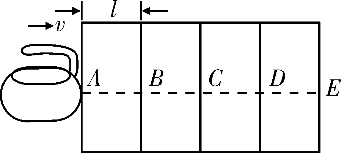
\includegraphics[width=50mm]{16.pdf}}%
\end{minipage}

\vfill


\newpage
\renewcommand{\solutiontitle}{{\bfseries 解: }}
{
\question  { \kaishu (本小题满分14分)}
	%\parpic(7cm,4cm)[r]{\includegraphics[width=6cm]{图17.pdf}}%

\begin{minipage}[t]{0.65\textwidth}
\linespread{1.4}\selectfont		
	{\CTEXindent
	如图,在平面直角坐标系$xOy$中,椭圆$C$:$\dfrac { x ^ { 2 } } { a ^ { 2 } } + \dfrac { y ^ { 2 } } { b ^ { 2 } } = 1 ( a > b > 0 )$的焦点为$F _ { 1 } ( - 1,0 )$,$F _ { 2 } ( 1,0 )$.过$F_2$作$x$轴的垂 线$l$,在$x$轴的上方,$l$与圆$F _2$:$( x - 1 ) ^ { 2 } + y ^ { 2 } = 4 a ^ { 2 }$交于点$A$,与椭圆$C$交于点$D$.连结$AF_1$并延长交圆$F_2$ 于点$B$,连结$BF_2$ 交椭圆$C$于点$E$,连接$DF _1$.已知$ DF_1=\dfrac{ 5}{2}$ .
	}
\begin{parts}
\part  
	求椭圆 $C$ 的标准方程;
\part  
	求点$ E$ 的坐标.
\end{parts}
	{\parpic{\includegraphics[width=8.4cm]{图17.pdf}}}%
\end{minipage} \quad
\begin{minipage}[t]{0.35\textwidth}
\vspace{-8pt}
	{\includegraphics[width=50mm]{1701.pdf}}%
\end{minipage}


\vfill


%\newpage
{
\question  { \kaishu (本小题满分16分)}

\begin{minipage}[t]{0.65\textwidth}
\linespread{1.4}\selectfont	
 	{\CTEXindent
	如图,一个湖的边界是圆心为 $O$ 的圆,湖的一侧有一条直线型公路 $l $,湖上有桥 $AB$($AB$ 是圆 $O$ 的直径).规划在 公路$ l$ 上选两个点$ P$、$Q$ ,并构建两段直线型道路 $PB$、$QA$ ,规划要求:线段 $PB$、$QA $上的所有点到点 O 的距离 均不小于圆$ O$ 的半径.已知点 $A$,$B$ 到直线$ l $的距离分别为$ AC$ 和 $BD $( $C$、$D$ 为垂足),测得
$AB = 10$, $AC = 6,$ $BD = 12$ (单位:百米).

	}
\begin{parts}
\part
	若道路 $PB$ 与桥 $AB$ 垂直,求道路$ PB $的长;
\part
	在规划要求下, $P $和 $Q $中能否有一个点选在$ D$ 处?并说明理由;	
\part
	在规划要求下,若道路 $PB $和$ QA$ 的长度均为 $d$ (单位:百米), 求当$ d $最小时,$ P$、$Q$ 两点间的距离.
\end{parts}
\end{minipage} \quad
\begin{minipage}[t]{0.35\textwidth}
\vspace{-8pt}
	{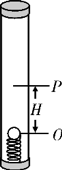
\includegraphics[width=50mm]{18.pdf}}%
\end{minipage}


\vfill


\newpage

\question  { \kaishu (本小题满分16分)} 
	
	{\CTEXindent
	设函数$f(x)=(x-a)(x-b)(x-c)$, $f'(x)$为$f(x)$的导函数.
	}
	
\begin{parts}
\part  
	若$a=b=c,f (4)=8$,求$a$的值;
\part 
	若 $a \ne b,b= c $,函数$ f (x)$和$ f '(x)$的零点均在集合$\set{-3,1,3}$中,求 $f(x)$的极小值;
\part 
	若$a = 0,0 < b \leqslant 1 , c = 1$,且$f(x)$的极大值为$M$,求证:$M \leqslant \dfrac { 4 } { 27 }$ .
\end{parts}
\vfill

%\newpage
\question  { \kaishu (本小题满分16分)}

	{\CTEXindent
	定义首项为 1 且公比为正数的等比数列为“ $M-$数列”.
	}
	
\begin{parts}
\part  
	已知等比数列$\left\{ a _ { n } \right\} \left( n \in \mathrm { N } ^ { * } \right)$满足:$a _ { 2 } a _ { 4 } = a _ { 5 } , a _ { 3 } - 4 a _ { 2 } + 4 a _ { 1 } = 0$,求证:数列$\left\{ a _ { n } \right\}$为“$M-$数列”;
\part
	已知数列$\left\{ b _ { n } \right\} \left( m \in \mathrm { N } ^ { * } \right)$满足:$b _ { 1 } = 1 , \dfrac { 1 } { S _ { n } } = \dfrac { 2 } { b _ { n } } - \dfrac { 2 } { b _ { n +1 } }$,其中$S_n$为数列$\left\{ b _ { n } \right\}$的前$n$项和.
	
	\dqsz{1}求数列 $\left\{ b _ { n } \right\}$的通项公式;
	
	\dqsz{2}设$m$为正整数,若存在“$M-$数列”$\left\{ c _ { n } \right\} \left( c \in \mathrm{N} ^ { * } \right)$,对任意正整数$k$,当$k \leqslant m$时,都有$c _ { k } \leqslant b _ { k } \leqslant c _ { k + 1 }$
	
	~\quad 成立,求$m$ 的最大值.
\end{parts}

\vfill
\end{questions}

\label{numpageA}
\newpage

\setcounter{page}{1}
\cfoot{\small \heiti{数学II (附加题)}\quad 第~\thepage~页(共 \numpages 页)}

\begin{center}
{ \bfseries \Large{2019年普通高等学校招生全国统一考试(江苏卷)}}
\end{center}
\begin{center}
{ \bfseries \Large{数学II(附加题)}}
\end{center}
%\vspace{-8ex}
%\begin{flushright}
%2011.6.7
%\end{flushright} 

%\noindent {\heiti 注意事项:}
%
%{\kaishu
%\indent	1. 本试卷共2页. 满分40分, 考试时间30分钟.  
%
%\indent	2. 请将解答题的解题过程写在答题卷的规定区域, 在本试卷上答题无效.  
%
%\indent   3. 答题前, 考生务必将自己的姓名、学校、考试号写在答题卷的规定位置.}

\noindent 
\fbox{%

\begin{minipage}[c][][c]{\textwidth}

\vspace{1ex}
\begin{center}
{ \bfseries \large{\heiti 注\quad 意\quad 事\quad 项}}
\end{center}

{\heiti 考生在答题前请认真阅读本注意事项及各题答题要求}


\begin{enumerate}

\item
	本试卷共2页,均为非选择题(第21题$\sim$第23题)。本卷满分为40分,考试时间为30分钟。考试结束后,请将本试卷和答题卡一并交回。
\item
	答题前,请您务必将自己的姓名、准考证号用0.5毫米黑色墨水的签字笔填写在试卷及答题卡的规定位置。
\item
	请认真核对监考员在答题卡上所粘贴的条形码上的姓名、准考证号与您本人是否相符。
\item
	作答试题,必须用0.5毫米黑色墨水的签字笔在答题卡上的指定位置作答,在其它位置作答一律无效。
\item
	如需作图,须用2B铅笔绘、写清楚,线条、符号等须加黑、加粗。
	
\end{enumerate}
\vspace{0.5ex}
\end{minipage}%
}%
\vspace{2ex}


\begin{questions}
\setcounter{question}{+20}

\question 
{\heiti 【选做题】本题包括A、B、C三小题,请\CJKunderdot{选定其中两题,并在相应的答题区域内作答}.若多做,则按作答的前两题评分.解答时应写出文字说明、证明过程或演算步骤.}
\renewcommand\thepartno{\Alph{partno}}
\renewcommand\partlabel{\thepartno.}
\renewcommand\thesubpart{\arabic{subpart}}
\renewcommand\subpartlabel{(\thesubpart)}

\begin{parts}
\renewcommand{\solutiontitle}{{\bfseries 证明:}}

\part{ [选修4 -- 2: 矩阵与变换]}{ (本小题满分10分)}

	已知矩阵$\mathbf{A} = \begin{bmatrix}
   3 & 1  \\
   2 & 2  \\
\end{bmatrix}$.

(1)求$\mathbf{A}^2$;

(2)求矩阵$\mathbf{A}$的特征值.

\vfill

%\newpage

\part {[选修4 -- 4: 坐标系与参数方程]}{  (本小题满分10分)}

	{\CTEXindent
	在极坐标系中,已知两点$A \left( 3 , \dfrac { \uppi } { 4 } \right) , B \left( \sqrt { 2 } , \dfrac { \uppi } { 2 } \right)$,直线 $l$的方程为$\rho \sin \left( \theta + \dfrac { \uppi } { 4 } \right) = 3$.
	}

(1)求 $A$,$ B$ 两点间的距离;

(2)求点$ B$ 到直线$l$的距离.

\vfill

\part {[选修4 -- 5: 不等式选讲]}
\renewcommand{\solutiontitle}{{\bfseries 解:}}
{ (本小题满分10分)}

	设 $x\in\mathrm{R}$,解不等式$| x | + | 2 x - 1 | > 2$.
	
\vfill

\end{parts}


\newpage

{\heiti 【必做题】第22题、第23题,每小题10分, 共计20分.请在\CJKunderdot{答题卡指定区域}内作答, 解答时应写出文字说明、证明过程或演算步骤. }
\renewcommand\thepartno{\arabic{partno}}
\renewcommand\partlabel{(\thepartno)}
\renewcommand\thesubpart{\roman{subpart}}
\renewcommand\subpartlabel{(\thesubpart)}

\renewcommand{\solutiontitle}{{\bfseries 解:}}

%\newpage
{
\question  { \kaishu (本小题满分10分)}
	
	{\CTEXindent
	设$( 1 + x ) ^ { n } = a _ { 0 } + a _ { 1 } x + a _ { 2 } x ^ { 2 } + \cdots + a _ { n } x ^ { n } , n \geqslant 4 , n \in \mathbf { N } ^ { * }$.已知$a _ { 3 } ^ { 2 } = 2 a _ { 2 } a _ { 4 }$.
	}
	
	(1)求 $n$ 的值;
	
	(2)设$( 1 + \sqrt { 3 } ) ^ { n } = a + b \sqrt { 3 }$, 其中 $a , b \in \mathbf { N } ^ { * }$,求$a ^ { 2 } - 3 b ^ { 2 }$的值.
	
\vfill

\newpage
%\renewcommand{\solutiontitle}{{\bfseries 证明:}}

\question  { \kaishu (本小题满分10分)}

	{\CTEXindent
	在平面直角坐标系 $xOy$ 中,设点集$A _ { n } = \set{ ( 0,0 ) , ( 1,0 ) , ( 2,0 ) , \cdots , ( n , 0 ) }$,$B _ { n } =\set{ ( 0,1 ) , ( n , 1 ) }$,
	
	$C _ { n } = \left\{ ( 0,2 ) , ( 1,2 ) , ( 2,2 ) , \cdots , ( n , 2 ) \}, n \in \mathbf { N } ^ { * } \right.$.令$M _ { n } = A _ { n } \cup B _ { n } \cup C _ { n }$.从集合 $M_n$中任取两个不同的点,用随机变量 $X$ 表示它们之间的距离.
	}
	
	(1)当 $n=1$ 时,求 $X$ 的概率分布;
	
	(2)对给定的正整数 $n ( n \geqslant 3 )$,求概率 $P ( X \leqslant n )$(用 $n$ 表示).
\vfill


\end{questions}

\end{document}

